\documentclass{maelab_y}
%\documentstyle{jarticle}
\usepackage{graphicx}
\usepackage[dvipdfmx]{color}
\usepackage{multirow}
\usepackage{here}

\newcommand{\figtb}[5]{ %引数 {日本語タイトル}{英語タイトル}{サイズ}{ファイル名}{ラベル名}
\begin{figure}[hbtp]
  \begin{center}
    \includegraphics[width=#3cm,clip]{figure/#4}
    \caption{#1}
    \label{fig:#5}
  \end{center}
\end{figure}}

\newcommand{\分類条件}{
\begin{table}[t]
\begin{center}
\caption{進行方向を分類する条件}
\ecaption{Classification condition of moving direction $e_{i}$.}
\label{tb:hantei_jouken}
\begin{tabular}{c|c|c|c|c}
\hline \hline
			& 右 & 左 & 上 & 下 \\ \hline
パターン2   & $\frac{1}{\sqrt{2}} < e_x \leq 1  $
		    & $ -1 \leq e_x < \frac{-1}{\sqrt{2}}$ 
		    & $ \frac{-1}{\sqrt{2}} < e_x < \frac{1}{\sqrt{2}} $ 
		    & $ \frac{-1}{2} < e_x < \frac{1}{2} $ \\
パターン3   & $\frac{-1}{2} < e_y < \frac{1}{2} $ 
		    & $\frac{-1}{2} < e_y < \frac{1}{2} $
            & $ \frac{1}{\sqrt{2}} < e_y \leq 1$
		    & $ -1 \leq e_y < \frac{-1}{\sqrt{2}} $ \\
\hline
\multirow{2}{*}{パターン4}   
			& $R_x \geq A_x$ & $R_x < A_x$ & $R_y \geq A_y$ & $R_y < A_y $ \\
	        &  $L_x \geq A_x$ & $L_x < A_x$ & $L_y \geq A_y$ & $L_y < A_y$ \\
\hline
\multirow{2}{*}{パターン5}   
 			& $R_x \geq x_1$ & $R_x < x_2$ & $R_y \geq y_1$ & $R_y < y_2 $ \\
			& $L_x \geq x_1$ & $L_x < x_2$ & $L_y \geq y_1$ & $L_y < y_2 $ \\
\hline
パターン6   & $ \cos(\frac{1}{2}\theta_{view}) \leq  e_y $ 
			& $ e_y \leq -\cos(\frac{1}{2}\theta_{view})$ 
			& $ \sin(\frac{1}{2}(\pi - \theta_{view})) \leq e_x $ 
			& $ e_x \leq \sin(\frac{1}{2}(\pi - \theta_{view}))  $ \\
\hline
\end{tabular}
\end{center}
\end{table}}

\newcommand{\距離計算回数}{
\begin{table}[hbtp]
\begin{center}
\caption{エージェント間距離の計算回数[$10^{10}$回]}
\label{tb:count_result_yobi}
\begin{tabular}{c|r|r|r|r|r|r}
\hline \hline
	%人数 & パターン1 & パターン2 & パターン3 & パターン4 & パターン5 & パターン6 \\  
	人数 & 1 & 2 & 3 & 4 & 5 & 6 \\  
	\hline
	\multirow{2}{*}{3000} 
	& 5.1   & $\mathbf{3.9}$   & 4.0    & 4.4    & 4.1    & 4.4   \\  
	&       & ($\mathbf{24.5}$\%) 					& (22.9\%) & (15.3\%) & (20.7\%) & (15.2\%) \\ \hline
	\multirow{2}{*}{5000} 
	& 14.4  &  $\mathbf{10.9}$  					  & 11.1   & 12.2   & 11.4   & 12.2  \\  
	&       & ($\mathbf{23.8}$\%) 					& (22.6\%) & (15.2\%) & (20.5\%) & (15.1\%) \\ \hline
	\multirow{2}{*}{7500} 
	& 33.1  & $\mathbf{25.2}$	 		    	 	 & 25.8   & 28.3   & 26.7   & 28.3  \\ 
	&       & ($\mathbf{23.9}$\%) 					& (22.2\%) & (14.6\%) & (19.4\%) & (14.6\%) \\ \hline
    \end{tabular}
  \end{center}
\end{table}}


\if 0
\usepackage[dvipdfmx]{graphicx}
\fi

\begin{document}
\title{進行方向の計算回数削減による
\\ソーシャルフォースモデルを用いた人流シミュレーションの高速化}
\学生番号{2281011}
\author{片寄\ 颯人}
\maketitle

\if 0
\section{はじめに}
駅や商業施設などのように人が多く集まる場所では,利便性や災害時の
安全性の観点から,混雑や滞留の対策が重要であり,
混雑や滞留の対策にソーシャルフォースモデル(SFM)を用いた
人流シミュレーションが広く用いられている\cite{helbing_sfm}.
SFMは,人を運動方程式に基づくエージェントとして再現するモデルである.
SFMを用いた人流シミュレーションは,解析規模に応じて,
エージェントの進行方向を決定する計算に時間がかかるため,
高速化が求められている.
そこで,本稿では,SFMを用いた人流シミュレーションを高速化するために,
進行方向計算中の演算回数を削減する手法を提案する.
\fi

\section{はじめに}
駅や商業施設などのように人が多く集まる場所では,利便性や災害時の
安全性の観点から,混雑や滞留の対策が重要であり,
混雑や滞留の対策にソーシャルフォースモデル(SFM)を用いた
人流シミュレーションが広く用いられている\cite{helbing_sfm}.
SFMは,人を運動方程式に基づくエージェントとして再現するモデルである.
SFMの運動方程式は,目的地に向かう力,周囲のエージェントや障害物を避ける力の
合力を用いてエージェントの移動を決定する.
SFMを用いた人流シミュレーションは,解析規模に応じて,
エージェントの進行方向を決定する計算に時間がかかるため,
高速化が求められている.
進行方向を決定する計算中の
目的地に向かう力と障害物を避ける力は,目的地と障害物の座標が変わらないため,
エージェントの座標に応じて決定する特徴がある.
そこで,本研究では,SFMを用いた人流シミュレーションを高速化するために,
解析領域を格子状に分割した領域ごとに目的地に向かう力と障害物を避ける力を
あらかじめ計算することで,解析中の進行方向計算中の演算回数を削減
する手法を提案する.

\section{ソーシャルフォースモデル(SFM)}
SFMは,時間ステップごとに各エージェントの進行方向を決定する運動方程式を
解くことで,人々の流れを再現する.
図\ref{fig:sfm_ex}にSFMのエージェント0の計算例を示す.
図中の四角は解析領域を分割したセル,赤丸は計算対象のエージェント,
黒丸は他のエージェント,色の付いた四角は判定に用いるセル(近似領域),
赤い点線は影響範囲を表す.
時刻$t$のエージェント$i$の進行方向は,
図\ref{fig:sfm_ex}のように,
自身の体重$m_i$,希望速度$v_i^0(t)$,現在速度$v_i(t)$,時定数$t_i$,
および,影響範囲内のエージェントを避ける力$f_{ij}$,
障害物を避ける力$f_{iW}$に基づいて算出する.
図\ref{fig:sfm_ex}の例では,エージェント0の進行方向を計算するとき,
色のついたセルに存在するエージェントに対して距離を計算し,
影響範囲内であるか判定する.
このとき,判定に用いるセルは,色の付いたセルであるため,白いセルに存在する
エージェントの影響範囲内であるかの判定を減らすことができる.

\begin{figure}[hbtp]
 \begin{center}
  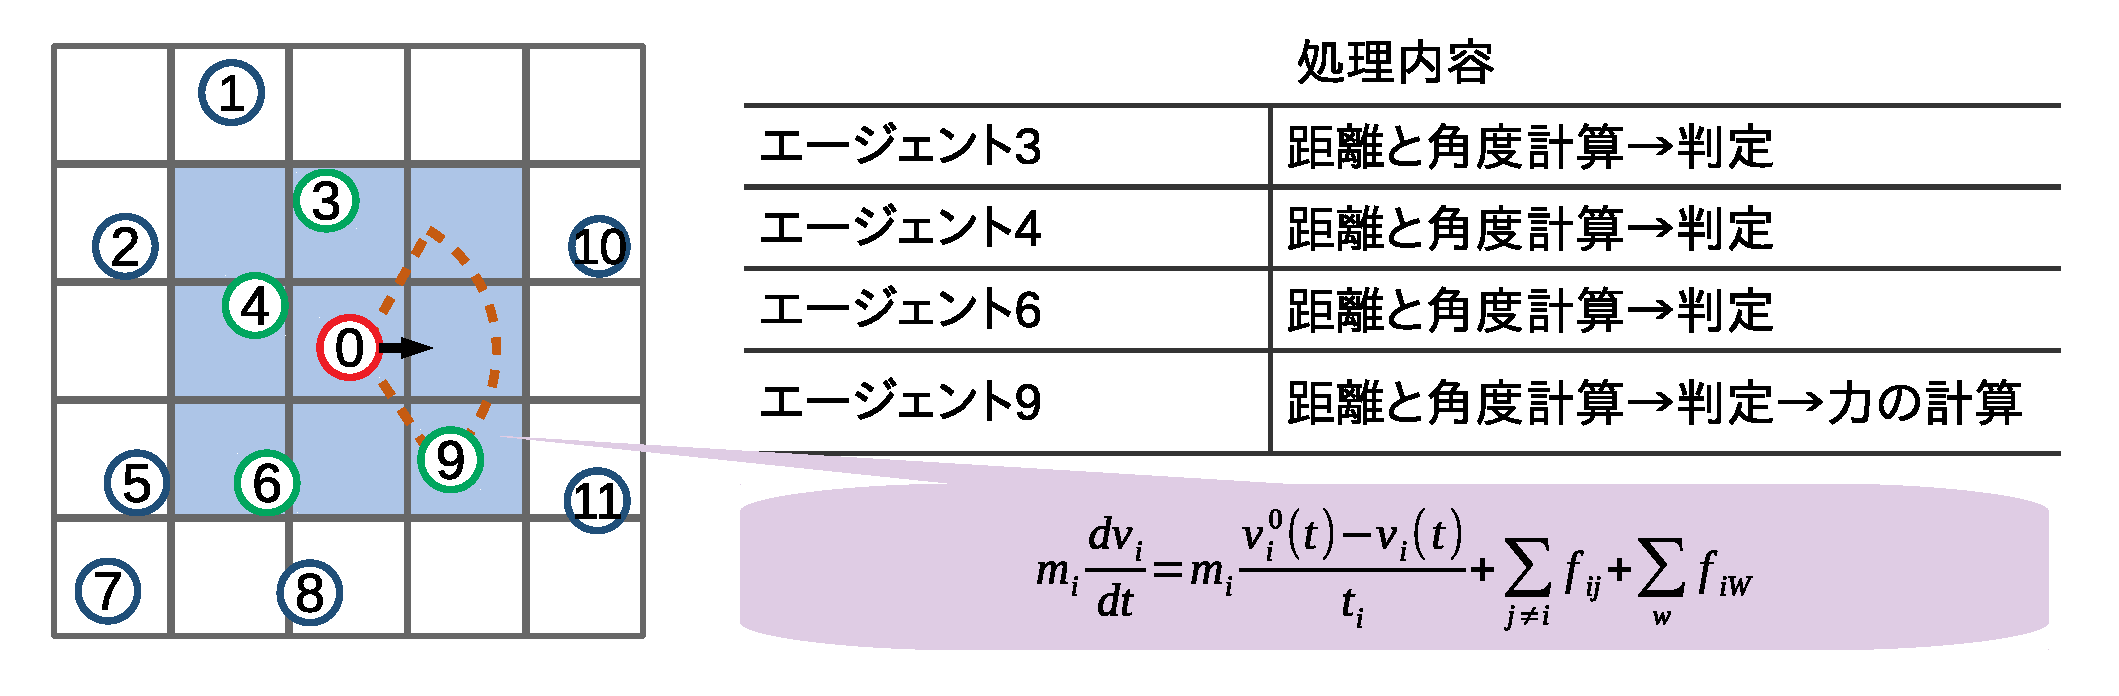
\includegraphics[width=7.21cm,clip]{figure/sfm_ex.eps}
  \caption{SFMの計算例}
  \label{fig:sfm_ex}
 \end{center}
\end{figure}

\section{進行方向計算中の演算回数削減手法}
SFMを用いた人流シミュレーションは,実問題に対して解析する場合,
エージェントや障害物が多く存在するため,進行方向の計算に時間がかかる.
目的地に向かう力と障害物を避ける力は,目的地と障害物の座標が
解析中に変わらないため,エージェントの座標に応じて決定する特徴がある.
また,エージェントを避ける力は,エージェント間距離に応じて決定する.
そこで,本研究では,解析領域を格子状に分割した領域ごとに,
目的地と障害物を避ける力をあらかじめ計算することで,
解析中の目的地に向かう力と障害物を避ける力の計算回数を削減する.
エージェントを避ける力は,エージェントの座標が解析中に変化することから,
あらかじめ計算できない.このため,提案手法は,
近似領域を影響範囲に高い精度で近似することで,
エージェントを避ける力の計算時のエージェント間距離の計算回数を削減する.


\figtb{進行方向ごとの近似領域}{}{7.5}{20220225_sentaku.eps}{sentaku}
\figtb{エージェント4の実装パターンごとの近似領域の例}{}{8}{20231007_hanni.eps}{90do_hamideru}


\section{エージェント間距離の計算回数削減手法}
FSFMは,視野の範囲がエージェントの進行方向前方の扇状の範囲であり,
後方のセルに存在する他のエージェントが視野の範囲内に存在するかという
の判定が不要になる.
正確に視野範囲のセルを選択するには,エージェントの座標や視野角度などの
情報から視野範囲を計算し,正確にセルを選択する必要があるので,時間がかかる.
そこで,本稿では,セルの選択にかかる処理時間を小さくするために,
図\ref{fig:teian_image}の5つのパターンを用いることで,
視野範囲内であるかの判定に用いるセルを削減し,FSFMを高速化する.
図\ref{fig:seru_ex1}の例では,提案手法のエージェントの進行方向から右の
削減パターンを適用することで,エージェント4,6とのエージェント間距離の
計算と視野範囲内かどうかの判定を減らすことができる.

\分類条件

\距離計算回数

\section{進行方向の計算回数削減手法}
aaaa

\section{評価}
提案手法の人流シミュレーションに対する有効性を確認するために,
セル分割法と提案手法のエージェント間計算回数と実行時間を測定する.
評価環境は,CPUがIntel Xeon E5-2687W v2,メモリが64GBである.
測定に用いる初期配置は,図\ref{fig:agent_haichi_image}に示すように,
交差と直進の配置である.
表\ref{tab:result}にセル分割法と提案手法の実行時間と高速化率,削減率を示す.
高速化率,削減率は式(\ref{eq:kousokukaritu}),
式(\ref{eq:sakugenritu})を用いる.
式(\ref{eq:kousokukaritu})中の$T_{k}$は既存手法の
エージェント間距離の計算回数,$T_{t}$は,提案手法の
エージェント間距離の計算回数である.

\begin{eqnarray}
  \label{eq:kousokukaritu}
  \mbox{高速化率[倍]} =
  \frac{\mbox{セル分割法の実行時間[s]}}{\mbox{提案手法の実行時間[s]}}
\end{eqnarray}

\begin{eqnarray}
  \label{eq:sakugenritu}
  \mbox{削減率[\%]} =
  \frac{T_{k} - T_{t}}{T_{k}} \times 100
\end{eqnarray}

表\ref{tab:result}より,提案手法は,既存手法よりも高速に解析
できることが確認できた.また,
提案手法のエージェント間距離の計算回数の
削減率は,交差の配置で約21\%,直進の配置で約31\%であり,
提案手法の高速化率は,既存手法に対して約1.5倍であることが
確認できた.これは,提案手法によるエージェント
間距離の計算回数が削減により,解析時間の短縮に繋がったから
と考えられる.また,直進の配置の方が削減率が高いのは,
後ろに近傍のエージェントが存在することが多いことが要因であると考えられる.

\if 0
\begin{figure}[hbtp]
 \begin{center}
  \includegraphics[draft, width=4.5cm,clip]{figure/kougai_haichi_2.eps}
  \caption{エージェントの初期配置}
  \label{fig:agent_haichi_image}
 \end{center}
\end{figure}
\fi

\begin{table}[hbtp]
  \begin{center}
    \caption{セル分割法と提案手法の実行時間と高速化率と削減率}
    \label{tab:result}
    \begin{tabular}{c|c|c|c|c}
      \hline \hline
        & 既存手法[s] & 提案手法[s] & 高速化率 & 削減率 \\
      \hline
      5000人交差 & \multicolumn{1}{|r|}{8321} &
       \multicolumn{1}{|r|}{5522} &
       \multicolumn{1}{|r|}{1.51} &
       \multicolumn{1}{|r}{21} \\
      \hline
      10000人交差 &
      \multicolumn{1}{|r|}{33898} &
      \multicolumn{1}{|r|}{22231} &
      \multicolumn{1}{|r|}{1.52}  &
      \multicolumn{1}{|r}{22} \\
      \hline
      5000人直進 &
      \multicolumn{1}{|r|}{29790} &
      \multicolumn{1}{|r|}{19337} &
      \multicolumn{1}{|r|}{1.54}  &
      \multicolumn{1}{|r}{31} \\
      \hline
      10000人直進 &
      \multicolumn{1}{|r|}{118212} &
      \multicolumn{1}{|r|}{77265} &
      \multicolumn{1}{|r|}{1.54} &
      \multicolumn{1}{|r}{31}  \\
      \hline
    \end{tabular}
  \end{center}
\end{table}

\section{おわりに}
本稿では,視野を用いた人流シミュレーションを高速化するために,
SFMのエージェント間距離の
計算回数を削減する手法を提案し,その有効性を評価した.評価の結果,提案手法の実行時間は,セル分割法に対して約1.5倍高速化することが確認できた.

\begin{thebibliography}{9}
\footnotesize
\bibitem{helbing_sfm}
  Helbing, D. and Molnar, P.: Social force model for pedestrian dynamics,{\em
    Physical review E}, Vol.~51, No.~5, p.\ 4282 (1995).

\bibitem{21_Isozaki}
  磯崎勝吾,中辻隆:Social force
  modelを基にした歩行者の避難シミュレーションモデルに関する研究,土木学会北海道支部論文報告集,
  Vol.~66 (2009).
\end{thebibliography}

\end{document}
